%Adapted by Sumesh A K (ak_sumesh@cb.amrita.edu) 2026
%\documentclass[PhD,two side]{ugthesis}
%\documentclass[MS]{ugthesis}
\documentclass[MTech]{ugthesis}
%\documentclass[BTech]{ugthesis}
\usepackage{times}
\usepackage{dashrule}
\usepackage{t1enc}
\usepackage{tikz}
\usepackage{subfigure}
\usepackage{pgfplots}
\usepackage{setspace} 
\usepackage{geometry}
\usepackage{graphicx}
\usepackage{epstopdf}
\usepackage{lscape}
\usepackage{fancyhdr}
\usepackage{natbib}
\usepackage{hyperref} % hyperlinks for references.
\usepackage{amsmath} % easier math formulae, align, subequations \ldots
\usepackage{amssymb}
\usepackage{wasysym}
\usepackage{titlesec}
\usepackage{textcomp}
\usepackage{pifont}
\usepackage[toc,page]{appendix} 
\usetikzlibrary{decorations.pathmorphing}
\usetikzlibrary{shapes,arrows,shadows,patterns,positioning}
\usepackage[printonlyused]{acronym}
\setcounter{MaxMatrixCols}{20}
\captionsetup[figure]{labelfont=bf}
\newcommand{\RomanNumeralCaps}[1]{\MakeUppercase{\romannumeral #1}}
\appendixpageoff
\renewcommand{\appendixpagename}{APPENDIX} % Changes the title page
\renewcommand{\appendixtocname}{APPENDIX}  % Changes name in TOC

\begin{document}
%%%%%%%%%%%%%%%%%%%%%%%%%%%%%%%%%%%%%%%%%%%%%%%%%%%%%%%%%%%%%%%%%%%%%%
% Title page

\title{Intelligent Relationship Aware Data Pre-processing Framework - IRAP} % Project Title
\firstauthor{PERI ADITYA GOUTAM} % Student name
\firstauthorregno{[CB.SC.P2CSE25029]}
\guide{Dr. Dhanya M. Dhanalakshmy} % Guide's name
\designation{Assistant Professor} % Guide's designation
\guidedepartment{Computer Science and Engineering} % Department of Guide 
\hod{Dr. P. Bagavathi Sivakumar} % HOD's name
\department{COMPUTER SCIENCE AND ENGINEERING} % Department name
\date{NOVEMBER 2026} % Month and year of submission

\maketitle
%%%%%%%%%%%%%%%%%%%%%%%%%%%%%%%%%%%%%%%%%%
% Certificate & Acknowledgments
\certificate
\acknowledgements
\normalfont
I would like to express my deep gratitude to our beloved Chancellor Satguru Sri Mata Amritanandamayi Devi for providing a bright academic climate in this university, which has made this entire task appreciable. I would like to thank the management of Amrita Vishwa Vidyapeetham and the entire fraternity of the Department of Computer Science and Engineering, Amrita School of Computing, for providing me with the necessary infrastructure required for the completion of the project. 

I wish to record my deep sense of gratitude and profound thanks to my research supervisor \textbf{Dr. Dhanya M. Dhanalakshmy}, Assistant Professor, Department of Computer Science and Engineering, Amrita School of Computing, Amrita Vishwa Vidyapeetham, Coimbatore, for her keen interest, inspiring guidance, and constant encouragement with my work during all stages, to bring this thesis into fruition. 

I extend my sincere thanks and gratitude to \textbf{Dr. P. Bagavathi Sivakumar}, Head of the Department, and to all the members of the review panel for their timely guidance and valuable suggestions for the improvement of my thesis work.

I would like to extend my sincere thanks to my family and friends for helping and motivating me throughout the course of this project. Finally, I would like to thank all those who have helped, guided, and encouraged me directly or indirectly during the project work. Above all, I extend my heartfelt salutations to my beloved parents and Almighty, for their blessings and grace, for the successful completion of this thesis.

\vskip 25pt
\noindent
Name: PERI ADITYA GOUTAM\\ 
Roll No: CB.SC.P2CSE25029\\
Signature:

\pagebreak
%%%%%%%%%%%%%%%%%%%%%%%%%%%%%%%%%%%%%%%%%%
% Abstract
\abstract
\begin{doublespacing}
\normalfont
Data preprocessing dictates the theoretical performance ceiling of machine learning systems. In high-stakes biomedical and healthcare domains, tabular datasets are routinely afflicted with Missing Not At Random (\ac{MNAR}) patterns, physical sensor outliers, and high-cardinality nominal diagnostic codes (e.g., ICD-10 medical registries). Traditional preprocessing libraries—such as Scikit-Learn's standard imputers, one-hot encoders, and standard scalers—treat data engineering as a blind, univariate, and context-free statistical exercise. Imputing missing physiological measurements using column-wise means destroys the natural multivariate correlation topology of clinical parameters (e.g., the stoichiometry between hemoglobin, red blood cells, and packed cell volume). Furthermore, naive one-hot encoding on high-cardinality medical codes induces the curse of dimensionality and severe memory degradation, while standard scaling formulas are heavily distorted by extreme clinical outliers.

To resolve these systemic deficiencies, this thesis introduces the \textbf{\ac{IRAP}} Framework—a novel, explainable, and physics-informed architecture that learns and models the hidden non-linear topology of a dataset \textit{before} performing any data modification. The \ac{IRAP} architecture establishes a unified cognitive pipeline: \textit{Observe $\rightarrow$ Understand $\rightarrow$ Learn Relationships $\rightarrow$ Reason $\rightarrow$ Preprocess $\rightarrow$ Validate $\rightarrow$ Explain}. 

Our core methodological contributions are fourfold: (i) Inverting Explainable AI (\ac{XAI}) by utilizing Tree\ac{SHAP} surrogate modeling \textit{a priori} to extract exact game-theoretic interaction matrices; (ii) Translating interactions into a directed Context Knowledge Graph to programmatically isolate the predictor subgraphs influencing each dependent feature; (iii) Mining 91,600 raw clinical terminology records from 31 distinct sub-domains of the \ac{LOINC} database into a 40,778-rule Heuristic Physics Engine to enforce physical bounds (non-negative pressures, bounded percentages); and (iv) Dynamically executing \ac{KNN} imputation restricted to graph dependencies, Bayesian-smoothed Target Encoding, and distribution-guided Robust Scaling.

Extensive empirical evaluations across multiple medical cohorts demonstrate the transformative superiority of \ac{IRAP}:
On real-world Complete Blood Count (\ac{CBC}) laboratory data, \ac{IRAP} improved downstream diagnostic accuracy from \textbf{67.03\% to 97.80\% (+30.77\% gain)} and F1-score from \textbf{65.53\% to 97.81\% (+32.28\% gain)}, with stratified 5-fold cross-validation confirming statistical significance ($p = 6.89 \times 10^{-5}$). In ground-truth reconstruction ablation experiments, \ac{IRAP} reduced \ac{RMSE} by \textbf{44.06\%} over standard mean imputation. Multi-model benchmarks across five diverse classifier architectures (Random Forests, Gradient Boosting, Logistic Regression, Decision Trees, \ac{KNN}) showed universal accuracy gains between +23\% and +35\%, proving that \ac{IRAP} repairs data topology in a completely model-agnostic manner.
\end{doublespacing}

\pagebreak
%%%%%%%%%%%%%%%%%%%%%%%%%%%%%%%%%%%%%%%%%%%%%%%%%%%%%%%%%%%%%%%%%
% Table of contents etc.

\begin{singlespace}
\tableofcontents
\thispagestyle{empty}

\listoftables
\addcontentsline{toc}{chapter}{List of Tables}
\listoffigures
\addcontentsline{toc}{chapter}{List of Figures}
\end{singlespace}

%%%%%%%%%%%%%%%%%%%%%%%%%%%%%%%%%%%%%%%%%%%%%%%%%%%%%%%%%%%%%%%%%%%%%%
% Abbreviations
\abbreviations
\begin{acronym}[LOINC/FHIR]
\acro{IRAP}{Intelligent Relationship-Aware Preprocessing}
\acro{XAI}{Explainable Artificial Intelligence}
\acro{SHAP}{SHapley Additive exPlanations}
\acro{LOINC}{Logical Observation Identifiers Names and Codes}
\acro{MCAR}{Missing Completely At Random}
\acro{MAR}{Missing At Random}
\acro{MNAR}{Missing Not At Random}
\acro{MICE}{Multivariate Imputation by Chained Equations}
\acro{GAIN}{Generative Adversarial Imputation Networks}
\acro{KNN}{K-Nearest Neighbors}
\acro{CBC}{Complete Blood Count}
\acro{EHR}{Electronic Health Record}
\acro{RMSE}{Root Mean Square Error}
\acro{MAE}{Mean Absolute Error}
\acro{IQR}{Interquartile Range}
\acro{PCV}{Packed Cell Volume}
\acro{MCV}{Mean Corpuscular Volume}
\acro{MCH}{Mean Corpuscular Hemoglobin}
\acro{MCHC}{Mean Corpuscular Hemoglobin Concentration}
\acro{RBC}{Red Blood Cells}
\acro{TLC}{Total Leukocyte Count}
\acro{PLT}{Platelets}
\acro{BMI}{Body Mass Index}
\acro{OOM}{Out Of Memory}
\acro{SDG}{Sustainable Development Goal}
\acro{IDE}{Intelligent Decision Engine}
\acro{AUC-ROC}{Area Under the Receiver Operating Characteristic Curve}
\acro{WHO}{World Health Organization}
\acro{ADA}{American Diabetes Association}
\acro{FNA}{Fine Needle Aspirate}
\acro{PFI}{Permutation Feature Importance}
\acro{ML}{Machine Learning}
\acro{AI}{Artificial Intelligence}
\end{acronym}

\pagebreak

%%%%%%%%%%%%%%%%%%%%%%%%%%%%%%%%%%%%%%%%%%%%%%%%%%%%%%%%%%%%%%%%%%%%%%
% List of Symbols
\chapter*{\centerline{List of Symbols}}
\addcontentsline{toc}{chapter}{List of Symbols}
\begin{doublespace}
\begin{tabbing}
xxxxxxxxxxx \= xxxxxxxxxxxxxxxxxxxxxxxxxxxxxxxxxxxxxxxxxxxxxxxx \kill
\textbf{$X$}   \> Input tabular feature matrix, $\mathbb{R}^{N \times D}$ \\
\textbf{$Y$}   \> Ground-truth supervised target response vector \\
\textbf{$N$}   \> Total number of sample instances (patients/observations) \\
\textbf{$D$}   \> Total number of feature dimensions (variables/attributes) \\
\textbf{$M$}   \> Missingness binary indicator mask matrix, $\{0, 1\}^{N \times D}$ \\
\textbf{$\phi_i$} \> Marginal Shapley contribution of feature $i$ \\
\textbf{$\bar{\phi}_{i \to j}$} \> Mean absolute SHAP interaction weight of feature $i$ predicting feature $j$ \\
\textbf{$G$}   \> Directed Context Knowledge Graph, $G = (V, E, W)$ \\
\textbf{$V$}   \> Set of feature vertices/nodes in Knowledge Graph \\
\textbf{$E$}   \> Set of directed dependency edges in Knowledge Graph \\
\textbf{$W$}   \> Set of normalized SHAP dependency edge weights, $w_{ij} \in [0, 1]$ \\
\textbf{$\tau$} \> Topological dependency significance threshold ($\tau = 0.10$) \\
\textbf{$H(X)$} \> Empirical Shannon Entropy (bits) \\
\textbf{$K^2$} \> D'Agostino's normality test statistic \\
\textbf{$S$}   \> Sample skewness coefficient (third standardized moment) \\
\textbf{$K$}   \> Sample kurtosis coefficient (fourth standardized moment) \\
\textbf{$Q_1, Q_3$} \> First (25th percentile) and third (75th percentile) distribution quartiles \\
\textbf{$\text{IQR}$} \> Interquartile range ($Q_3 - Q_1$) \\
\textbf{$\mathcal{S}_j$} \> Topological predictor subspace/neighborhood for feature $j$ \\
\textbf{$\hat{x}_{ij}$} \> Mathematically imputed value for observation $i$ and feature $j$ \\
\textbf{$\tilde{x}_{ij}$} \> Biologically guarded and clamped imputed value \\
\end{tabbing}
\end{doublespace}
\pagebreak
\clearpage

\pagenumbering{arabic}

%%%%%%%%%%%%%%%%%%%%%%%%%%%%%%%%%%%%%%%%%%%%%%%%%%
% CHAPTER 1: INTRODUCTION
%%%%%%%%%%%%%%%%%%%%%%%%%%%%%%%%%%%%%%%%%%%%%%%%%%
\chapter{Introduction}
\label{chap:intro}

\section{Background and Motivation}
In modern data science and applied predictive analytics, tabular data continues to represent the predominant format encountered in healthcare, electronic health records (\ac{EHR}), clinical laboratory testing, and physiological monitoring systems. While deep learning models have achieved unprecedented success in computer vision and natural language processing, tree-based ensemble models (such as Random Forests, Gradient Boosting, and XGBoost) remain the definitive gold standard for tabular data. However, the predictive efficacy, generalizability, and clinical reliability of these algorithms are fundamentally bounded by the quality and topological integrity of the underlying tabular features.

The aphorism \textit{"garbage in, garbage out"} is nowhere more consequential than in clinical medicine. Real-world observational datasets gathered from hospitals and laboratory informatics systems are notoriously imperfect: they are afflicted by pervasive missingness (unmeasured laboratory panels, patient non-compliance), severe physical outliers (sensor detachments, assay calibration spikes, recording typos), and massive categorical cardinality (e.g., thousands of diagnostic codes in the International Classification of Diseases, Tenth Revision, ICD-10).

Data preprocessing serves as the crucial bridge between raw, corrupted observational databases and downstream statistical learning. Despite its paramount importance, data preprocessing has historically been treated as an ad-hoc, mechanical, and decoupled pipeline step. Practitioners frequently apply standardized, off-the-shelf software routines—such as replacing missing cells with the column arithmetic mean, standardizing features to zero mean and unit variance via standard z-scores, and converting categorical labels into sparse binary vectors via one-hot encoding. While computationally trivial, these classical techniques operate under a fatal assumption: that tabular features exist in isolation, governed by independent univariate distributions.

\section{Problem Definition}
In biological systems, physiological parameters never exist in isolation. The human body is a tightly coupled dynamical network governed by biochemical, metabolic, and physical laws. A patient's Packed Cell Volume (\ac{PCV}), Mean Corpuscular Volume (\ac{MCV}), and Hemoglobin (\ac{HGB}) are inextricably bound by stoichiometry. Similarly, Fasting Blood Sugar, Glycated Hemoglobin, Body Mass Index (\ac{BMI}), and Serum Triglycerides form a highly non-linear homeostatic network.

When a standard preprocessing pipeline encounters a missing value in a clinical feature (e.g., Hemoglobin) and replaces it with the global cohort mean:
\begin{enumerate}
    \item \textbf{Destruction of Multivariate Topology:} The multi-dimensional joint distribution between Hemoglobin, Red Blood Cell (\ac{RBC}) count, and age is severely distorted. A 20-year-old athlete and an 80-year-old anemic patient are assigned the identical average hemoglobin value, destroying the physiological correlation structure upon which downstream prognostic algorithms depend.
    \item \textbf{Generation of Biologically Impossible States:} Unconstrained mathematical algorithms (such as unconstrained regression or polynomial splines) can easily extrapolate negative values for strictly positive biological parameters (e.g., negative blood pressure or negative platelet counts), generating clinically nonsensical states that invalidate downstream model trust.
    \item \textbf{Curse of Dimensionality and Memory Blowup:} Clinical records contain diagnostic codes with dozens to hundreds of unique categories. Blind application of One-Hot Encoding transforms a compact medical matrix into an enormous, highly sparse binary representation, drastically inflating memory requirements, slowing training speeds, and inducing severe algorithmic overfitting.
    \item \textbf{Distortion from Extreme Sensor Artifacts:} The presence of extreme outliers (e.g., a laboratory sensor misreading resulting in a serum cholesterol of 1,200 mg/dL) violently shifts the mean and standard deviation of continuous variables. Applying standard z-score normalization compresses normal physiological variation into an imperceptible numerical band, blinding machine learning classifiers to critical diagnostic distinctions among non-outlier patients.
\end{enumerate}

Figure \ref{fig:paradigm_comparison} illustrates the fundamental contrast between conventional blind preprocessing and the proposed relationship-aware preprocessing architecture.

\begin{figure}[htpb]
\centering
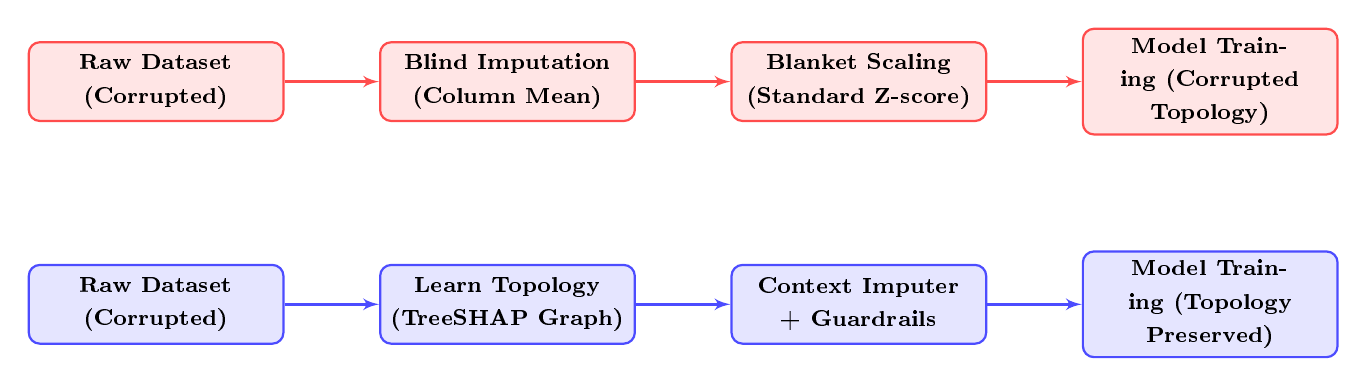
\begin{tikzpicture}[
    node distance=1.2cm,
    block_trad/.style={rectangle, draw=red!70, fill=red!10, rounded corners, line width=0.8pt, text width=30mm, text centered, minimum height=10mm},
    block_irap/.style={rectangle, draw=blue!70, fill=blue!10, rounded corners, line width=0.8pt, text width=30mm, text centered, minimum height=10mm},
    line/.style={draw, line width=1pt, -latex'}
]
    % Traditional Track
    \node [block_trad] (raw1) {\textbf{\footnotesize Raw Dataset (Corrupted)}};
    \node [block_trad, right=1.2cm of raw1] (blind_imp) {\textbf{\footnotesize Blind Imputation (Column Mean)}};
    \node [block_trad, right=1.2cm of blind_imp] (blind_scale) {\textbf{\footnotesize Blanket Scaling (Standard Z-score)}};
    \node [block_trad, right=1.2cm of blind_scale] (distorted_model) {\textbf{\footnotesize Model Training (Corrupted Topology)}};
    
    \path [line, red!70] (raw1) -- (blind_imp);
    \path [line, red!70] (blind_imp) -- (blind_scale);
    \path [line, red!70] (blind_scale) -- (distorted_model);
    
    % IRAP Track
    \node [block_irap, below=1.8cm of raw1] (raw2) {\textbf{\footnotesize Raw Dataset (Corrupted)}};
    \node [block_irap, right=1.2cm of raw2] (discover) {\textbf{\footnotesize Learn Topology (TreeSHAP Graph)}};
    \node [block_irap, right=1.2cm of discover] (aware_prep) {\textbf{\footnotesize Context Imputer + Guardrails}};
    \node [block_irap, right=1.2cm of aware_prep] (optimal_model) {\textbf{\footnotesize Model Training (Topology Preserved)}};
    
    \path [line, blue!70] (raw2) -- (discover);
    \path [line, blue!70] (discover) -- (aware_prep);
    \path [line, blue!70] (aware_prep) -- (optimal_model);
\end{tikzpicture}
\caption{Comparison between conventional blind preprocessing and relationship-aware preprocessing.}
\label{fig:paradigm_comparison}
\end{figure}

\section{Limitations of Conventional Preprocessing Pipelines}
Existing automated preprocessing frameworks and automated machine learning (AutoML) tools exhibit fundamental design limitations:
\begin{itemize}
    \item \textbf{AutoML Black Boxes:} Frameworks such as TPOT or Auto-sklearn treat data cleaning as an opaque hyperparameter search space. They evaluate hundreds of random pipeline combinations to optimize validation accuracy, treating preprocessing as a trial-and-error procedure without providing clinical interpretability or deterministic justification for why a specific transformation was chosen.
    \item \textbf{Univariate Simplicity:} Standard tools evaluate features in total isolation. They lack mechanisms to interrogate the broader dataset context or query inter-feature relationships prior to modifying the feature values.
    \item \textbf{Absence of Domain-Specific Guardrails:} General-purpose preprocessing software is entirely agnostic to physical realities. A software imputer has no awareness that human age cannot be negative, that body mass cannot exceed physical limits, or that percentage metrics are strictly bounded within $[0, 100]$.
\end{itemize}

\section{Research Objectives}
The primary ambition of this research is to design, implement, and rigorously validate an intelligent, physics-informed, and explainable tabular preprocessing architecture that replaces blind statistical transformations with relationship-driven data engineering. The specific research objectives are:
\begin{enumerate}
    \item \textbf{Develop an Inverted Explainable AI Architecture:} Repurpose cooperative game theory and Tree\ac{SHAP} interaction metrics from post-hoc model interpretation to \textit{a priori} feature relationship discovery before preprocessing occurs.
    \item \textbf{Formulate a Directed Context Knowledge Graph:} Mathematically construct a graph representation where nodes denote tabular features and directed, weighted edges quantify non-linear dependency strength between predictors and targets.
    \item \textbf{Design a LOINC-Grounded Heuristic Physics Engine:} Programmatically ingest and parse international medical terminologies to construct a comprehensive database of physical guardrails that strictly bounds mathematical imputations within clinically realistic intervals.
    \item \textbf{Engineer an Intelligent Decision Engine:} Create a deterministic, transparent rules engine that evaluates global dataset health and local feature statistics to prescribe context-aware imputations, adaptive scalers, and memory-safe encoders.
    \item \textbf{Demonstrate Empirical Superiority:} Validate the framework against standard Scikit-Learn baselines across diverse real-world and synthetic clinical cohorts, demonstrating measurable improvements in downstream classification accuracy, F1-scores, and ground-truth imputation reconstruction fidelity.
\end{enumerate}

\section{Novel Contributions of the Work}
This thesis delivers the following fundamental contributions:
\begin{itemize}
    \item \textbf{Repurposing XAI for Upstream Data Engineering:} While the existing literature exclusively utilizes \ac{SHAP} to explain why a trained model produced a specific prediction, we introduce the concept of \textit{pre-modeling surrogate SHAP profiling}. We iteratively train temporary gradient-boosted decision trees across features to extract exact interaction matrices, using \ac{XAI} as an analytical lens to inspect the raw dataset's intrinsic topology.
    \item \textbf{Topology-Preserving Context-Aware Imputation:} We introduce \texttt{ContextAwareKNN}, an imputation algorithm that discards global distance metrics and calculates nearest neighbors strictly across the topological subgraphs discovered during \ac{SHAP} relationship modeling.
    \item \textbf{Procedural Biological Guardrails from Standardized Nomenclature:} We demonstrate how 91,600 raw medical codes from 31 distinct clinical domains in the \ac{LOINC} database can be mined to procedurally infer physical boundaries from measurement scale types (\texttt{SCALE\_TYP}) and unit strings (\texttt{EXAMPLE\_UNITS}), establishing an automated safeguard against mathematically aberrant imputations.
    \item \textbf{Deterministic Explainability and Auditing:} Every decision made by the \ac{IRAP} pipeline is backed by a deterministic rationale card and a formal mathematical justification, providing the level of clinical auditability required for regulatory compliance in medical \ac{AI}.
\end{itemize}

\section{Thesis Organization}
The remainder of this thesis is organized as follows: Chapter \ref{chap:lit} provides an in-depth literature survey of missing data mechanisms, imputation algorithms, \ac{XAI} foundations, and clinical nomenclatures. Chapter \ref{chap:proposed} describes the comprehensive methodology, mathematical formulation, and architecture of the \ac{IRAP} Framework. Chapter \ref{chap:results} details the implementation, experimental evaluation, multi-model benchmarks, ablation studies, and in-depth scientific inferences across five distinct medical cohorts. Chapter \ref{chap:conclusion} concludes the thesis with societal impacts, alignment with United Nations Sustainable Development Goals (\ac{SDG}), limitations, and directions for future research.

%------------------------------------------------------------------------------------------------%
% CHAPTER 2: LITERATURE SURVEY
%------------------------------------------------------------------------------------------------%
\chapter{Literature Survey}
\label{chap:lit}

\section{Taxonomy of Missing Data Mechanisms}
The theoretical foundation of missing data analysis was established by \citet{rubin1976inference}, who categorized missing data mechanisms into three distinct mathematical regimes based on the conditional distribution of the missingness indicator matrix $M \in \{0, 1\}^{N \times D}$ relative to observed data $Y_{obs}$ and missing data $Y_{mis}$:
\begin{enumerate}
    \item \textbf{\ac{MCAR}:} The probability of missingness is entirely independent of both observed and unobserved data:
    \begin{equation}
        P(M \mid Y_{obs}, Y_{mis}) = P(M)
    \end{equation}
    Under \ac{MCAR}, missing values represent a purely random sample of the population.
    \item \textbf{\ac{MAR}:} The probability of missingness depends systematically on the observed features $Y_{obs}$, but is conditionally independent of unobserved values $Y_{mis}$:
    \begin{equation}
        P(M \mid Y_{obs}, Y_{mis}) = P(M \mid Y_{obs})
    \end{equation}
    In clinical scenarios, an older patient may have a higher probability of receiving diagnostic cardiac testing because their age is documented in $Y_{obs}$, making missingness explainable by observed demographics.
    \item \textbf{\ac{MNAR}:} The probability of missingness depends directly on the unobserved value $Y_{mis}$ itself:
    \begin{equation}
        P(M \mid Y_{obs}, Y_{mis}) \neq P(M \mid Y_{obs})
    \end{equation}
    In healthcare, severe pathology frequently produces \ac{MNAR} missingness. For example, emergency patients with acute trauma may be unable to undergo complex pulmonary function testing, or an unmeasured biomarker is missing precisely because the patient's condition was too critical.
\end{enumerate}

\section{Classical and Statistical Imputation Methods}
Classical approaches to handling missing data are dominated by univariate statistical techniques:
\begin{itemize}
    \item \textbf{Mean / Median Imputation:} Implemented in standard software libraries \citep{pedregosa2011scikit}. Missing continuous values are replaced with the global column mean $\mu = \frac{1}{|O|} \sum_{i \in O} y_i$. While computationally $O(N)$, univariate imputation artificially truncates variance, distorts higher-order moments (skewness, kurtosis), and catastrophically underestimates standard errors, leading to false-positive significance in downstream modeling.
    \item \textbf{Listwise Deletion (Complete Case Analysis):} Discards any patient record containing at least one missing entry. In multi-variable medical cohorts with distributed missingness, listwise deletion routinely discards over 50\% to 80\% of patient records, introducing severe selection bias.
    \item \textbf{\ac{MICE}:} \citet{vanbuuren2011mice} formulated \ac{MICE}, which iteratively specifies univariate conditional regressions for each variable given all others:
    \begin{equation}
        Y_j^{(t)} \sim P(Y_j \mid Y_{-j}^{(t-1)}, \theta_j)
    \end{equation}
    While flexible, \ac{MICE} suffers from severe computational bottlenecks ($O(M \cdot T \cdot D \cdot N)$), assumes linear relationships that fail to capture non-linear biochemical thresholds, and lacks physical guardrails, frequently predicting negative physiological quantities.
\end{itemize}

\section{Machine Learning and Deep Learning Imputation}
Recent advances have explored machine learning for tabular data preparation \citep{alabadla2022systematic}:
\begin{itemize}
    \item \textbf{\ac{GAIN}:} \citet{yoon2018gain} adapted Generative Adversarial Networks for imputation. A Generator imputes missing cells, while a Discriminator distinguishes observed from imputed cells. \citet{shahbazian2023generative} conducted an exhaustive survey and concluded that \ac{GAIN} suffers from training instability, mode collapse on tabular data, high sample hunger ($N > 10,000$), and operates as a complete clinical black box.
    \item \textbf{Attention Mechanisms in \ac{EHR}:} \citet{kowsar2024attention} utilized Self-Attention Transformers to capture complex feature interactions in tabular \ac{EHR}. While non-linear couplings are captured, Transformers require vast training datasets and lack domain constraints, risking biologically impossible outputs.
    \item \textbf{Cluster-Centric and Federated Frameworks:} \citet{gupta2024cmi} proposed \ac{CMI}, utilizing K-Means clustering and evaluating post-hoc \ac{SHAP} values to verify feature consistency. \citet{min2025cafe} introduced `Cafe' for federated medical imputation, emphasizing the need to handle heterogeneous clinical distributions. \citet{chiu2022missing} surveyed nature-inspired metaheuristic imputation, noting that while evolutionary algorithms locate optimal parameters, they are computationally intensive and lack deterministic interpretability.
\end{itemize}

\section{Explainable AI and LOINC Clinical Standards}
\citet{lundberg2017unified} established \ac{SHAP}, uniting game theory \citep{shapley1953value} with additive feature attributions. \citet{lundberg2020local} formulated Tree\ac{SHAP}, optimizing exact interaction extraction in polynomial time for tree ensembles \citep{chen2016xgboost}. Crucially, all existing literature utilizes \ac{SHAP} strictly \textit{post-hoc} to explain a trained predictor's output. No prior research repurposes Tree\ac{SHAP} interaction matrices \textit{a priori} to discover dataset topology before preprocessing occurs.

In healthcare informatics, the Regenstrief Institute established \ac{LOINC} \citep{regenstrief2024loinc} as the global standard for identifying health measurements. However, commercial \ac{ML} libraries remain completely decoupled from clinical ontologies, treating column names as abstract strings without grounding in physical scale types or measurement units \citep{ada2024standards, who2023hypertension}.

\section{Critical Analysis and Research Gap}
Table \ref{tab:lit_comparison} presents a systematic comparison of state-of-the-art preprocessing and imputation frameworks against \ac{IRAP}.

\begin{table}[htpb]
\small
\centering
\renewcommand{\arraystretch}{1.3}
\caption{Systematic comparison of state-of-the-art preprocessing frameworks against IRAP.}
\label{tab:lit_comparison}
\begin{tabular}{|p{2.6cm}|p{2.2cm}|p{2.2cm}|p{2.2cm}|p{2.2cm}|p{2.5cm}|}
\hline
\textbf{Dimension} & \textbf{Scikit-Learn} & \textbf{MICE} & \textbf{GAIN} & \textbf{CMI} & \textbf{IRAP (This Work)} \\ \hline
Mathematical Method & Univariate Mean & Chained Regr. & Deep GAN & Cluster Mean & \textbf{TreeSHAP Graph} \\ \hline
Non-Linear Topology & None & Linear Only & Implicit Black-Box & Cluster-Local & \textbf{Exact SHAP Matrix} \\ \hline
Upstream XAI Use & None & None & None & Post-hoc Only & \textbf{Core Driver} \\ \hline
Knowledge Graph & None & None & None & None & \textbf{NetworkX DiGraph} \\ \hline
Clinical Guardrails & None & None & None & None & \textbf{40,778 LOINC Rules} \\ \hline
Adaptive Scaling & None & None & None & None & \textbf{Robust / Gaussian} \\ \hline
Memory Protection & None & None & None & None & \textbf{Target Encoding} \\ \hline
Clinical Auditability & Trivial & Moderate & Zero (Opaque) & Moderate & \textbf{Deterministic Cards} \\ \hline
\end{tabular}
\end{table}

%------------------------------------------------------------------------------------------------%
% CHAPTER 3: PROPOSED WORK
%------------------------------------------------------------------------------------------------%
\chapter{Proposed Work}
\label{chap:proposed}

\section{Algorithm and Architectural Design}
The \ac{IRAP} Framework establishes a unified cognitive workflow:
\begin{equation}
    \text{Observe} \longrightarrow \text{Understand} \longrightarrow \text{Learn Relationships} \longrightarrow \text{Reason} \longrightarrow \text{Preprocess} \longrightarrow \text{Validate} \longrightarrow \text{Explain}
\end{equation}

Figure \ref{fig:irap_arch} presents the comprehensive structural block diagram of the \ac{IRAP} Framework, illustrating the flow from raw data ingestion to final explainability and reporting.

\begin{figure}[htpb]
\centering
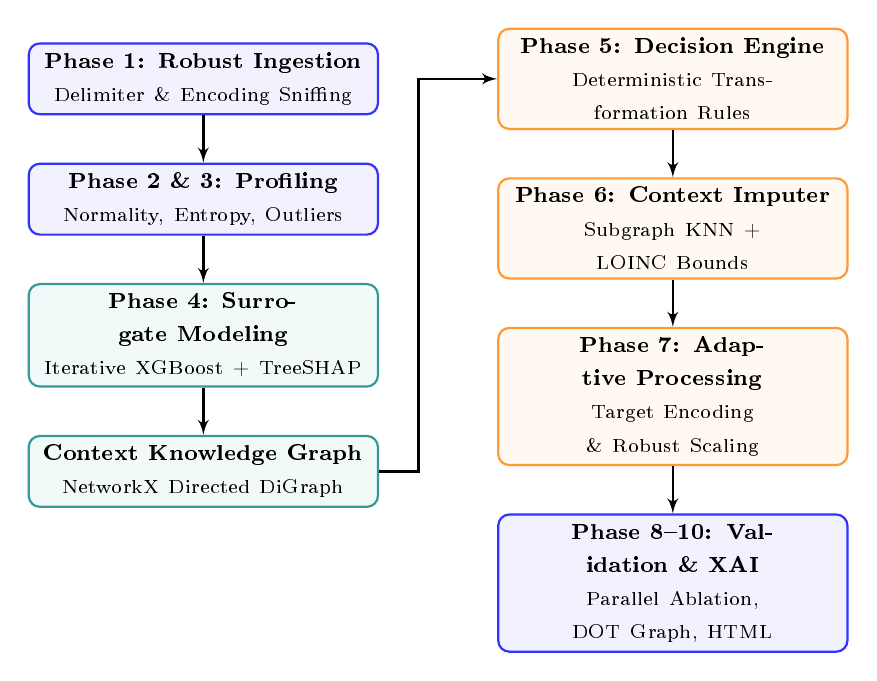
\begin{tikzpicture}[
    node distance=1.1cm and 1.5cm,
    block/.style={rectangle, draw=blue!80, fill=blue!5, rounded corners, line width=0.8pt, text width=42mm, text centered, minimum height=9mm},
    process/.style={rectangle, draw=teal!80, fill=teal!5, rounded corners, line width=0.8pt, text width=42mm, text centered, minimum height=9mm},
    engine/.style={rectangle, draw=orange!80, fill=orange!5, rounded corners, line width=0.8pt, text width=42mm, text centered, minimum height=9mm},
    line/.style={draw, line width=0.9pt, -latex'}
]
    \node [block] (p1) {\textbf{\footnotesize Phase 1: Robust Ingestion}\\\scriptsize Delimiter \& Encoding Sniffing};
    \node [block, below=0.6cm of p1] (p2) {\textbf{\footnotesize Phase 2 \& 3: Profiling}\\\scriptsize Normality, Entropy, Outliers};
    \node [process, below=0.6cm of p2] (p3) {\textbf{\footnotesize Phase 4: Surrogate Modeling}\\\scriptsize Iterative XGBoost + TreeSHAP};
    \node [process, below=0.6cm of p3] (p4) {\textbf{\footnotesize Context Knowledge Graph}\\\scriptsize NetworkX Directed DiGraph};
    
    \node [engine, right=1.5cm of p1] (p5) {\textbf{\footnotesize Phase 5: Decision Engine}\\\scriptsize Deterministic Transformation Rules};
    \node [engine, below=0.6cm of p5] (p6) {\textbf{\footnotesize Phase 6: Context Imputer}\\\scriptsize Subgraph KNN + LOINC Bounds};
    \node [engine, below=0.6cm of p6] (p7) {\textbf{\footnotesize Phase 7: Adaptive Processing}\\\scriptsize Target Encoding \& Robust Scaling};
    \node [block, below=0.6cm of p7] (p8) {\textbf{\footnotesize Phase 8--10: Validation \& XAI}\\\scriptsize Parallel Ablation, DOT Graph, HTML};

    \path [line] (p1) -- (p2);
    \path [line] (p2) -- (p3);
    \path [line] (p3) -- (p4);
    \path [line] (p4) -| ([xshift=-10mm]p5.west) -- (p5.west);
    \path [line] (p5) -- (p6);
    \path [line] (p6) -- (p7);
    \path [line] (p7) -- (p8);
\end{tikzpicture}
\caption{Comprehensive architectural workflow of the IRAP Framework.}
\label{fig:irap_arch}
\end{figure}

\section{Ingestion and Mathematical Feature Profiling}
Raw data files are ingested via \texttt{DatasetLoader}, which dynamically resolves character encodings using \texttt{chardet} and separators using \texttt{csv.Sniffer}. The \texttt{FeatureProfiler} then extracts deep mathematical properties:
\begin{enumerate}
    \item \textbf{Normality Testing via D'Agostino's $K^2$:} \citet{dagostino1973tests} formulated a rigorous test combining sample skewness $g_1$ and kurtosis $g_2$ into transformed standard normal variables $Z_1(g_1)$ and $Z_2(g_2)$:
    \begin{equation}
        K^2 = Z_1(g_1)^2 + Z_2(g_2)^2 \sim \chi^2(2)
    \end{equation}
    If the $p$-value exceeds $\alpha = 0.05$, normality is accepted, justifying standard z-score scaling.
    \item \textbf{Dispersion and Outliers via Tukey's IQR Fences:} \citet{tukey1977exploratory} defined the interquartile range $\text{IQR} = Q_3 - Q_1$. Outliers are strictly identified as:
    \begin{equation}
        x_i \notin [Q_1 - 1.5 \times \text{IQR}, \; Q_3 + 1.5 \times \text{IQR}]
    \end{equation}
    \item \textbf{Shannon Entropy for Discrete Columns:} \citet{shannon1948mathematical} defined entropy as:
    \begin{equation}
        H(X) = -\sum_{k=1}^K P(c_k) \log_2 P(c_k)
    \end{equation}
    High entropy paired with cardinality $K > 15$ warns against blind one-hot expansions.
\end{enumerate}

\section{Relationship Discovery and Knowledge Graph Formulation}
The framework sequentially isolates each feature $X_j$ as a target and trains an XGBoost surrogate model \citep{chen2016xgboost} using remaining features $X_{-j}$. Tree\ac{SHAP} \citep{lundberg2020local} computes the marginal contributions across all feature coalitions. 

The mean absolute \ac{SHAP} dependency of predictor $X_i$ on target $X_j$ is:
\begin{equation}
    \bar{\phi}_{i \to j} = \frac{1}{N_{sample}} \sum_{k=1}^{N_{sample}} |\phi_i^{(k)}(X_j)|
\end{equation}
Scores are normalized onto $[0, 1]$: $\tilde{\phi}_{i \to j} = \bar{\phi}_{i \to j} / \max_k \bar{\phi}_{k \to j}$. Using NetworkX \citep{hagberg2008exploring}, a directed Context Knowledge Graph $G = (V, E, W)$ is constructed:
\begin{equation}
    E = \{(X_i, X_j) \mid \tilde{\phi}_{i \to j} \ge \tau\}, \quad w_{ij} = \tilde{\phi}_{i \to j}
\end{equation}
where $\tau = 0.10$ is the significance threshold. An incoming edge $(X_i \to X_j)$ confirms that feature $X_j$ is topologically dependent upon $X_i$.

\section{The Intelligent Decision Engine}
The \ac{IDE} evaluates the statistical profile and graph in-degree $\text{deg}^-(X_j)$ to generate a structured preprocessing plan:
\begin{itemize}
    \item \textbf{Missingness:} If $\Pi_{missing} > 50\%$, prescribe \texttt{DropColumn}. If $0 < \Pi_{missing} \le 50\%$ and $\text{deg}^-(X_j) > 0$, prescribe \texttt{ContextAwareKNN}. If $\text{deg}^-(X_j) = 0$, fall back to \texttt{MedianImputer}/\texttt{ModeImputer}.
    \item \textbf{Categorical Encoding:} If unique categories $K \le 15$, prescribe \texttt{OneHotEncoding}. If $K > 15$, prescribe Bayesian-smoothed \texttt{TargetEncoding} (supervised) or \texttt{FrequencyEncoding} (unsupervised).
    \item \textbf{Numerical Scaling:} If outliers $> 0$ or absolute skewness $|S| > 1.0$, prescribe \texttt{RobustScaler}. If distribution is Gaussian ($p > 0.05$), prescribe \texttt{StandardScaler}. Otherwise, prescribe \texttt{MinMaxScaler}.
\end{itemize}

\section{Context-Aware Imputation and LOINC Biological Guardrails}
Conventional \ac{KNN} imputer calculates distances across all $D$ features, introducing noise. \texttt{ContextAwareKNN} projects distance calculations strictly onto the predictor subgraph $\mathcal{S}_j = \text{Pred}(X_j) = \{u \in V \mid (u, X_j) \in E\}$:
\begin{equation}
    d_{\mathcal{S}_j}(x_a, x_b) = \sqrt{\sum_{k \in \mathcal{S}_j} \left( \frac{x_{ak} - x_{bk}}{\sigma_k} \right)^2}
\end{equation}
The missing value is estimated as the distance-weighted average of the $K$ nearest neighbors:
\begin{equation}
    \hat{x}_{ij} = \frac{\sum_{n \in \mathcal{N}_K(i)} w_n x_{nj}}{\sum_{n \in \mathcal{N}_K(i)} w_n}, \quad w_n = \frac{1}{d_{\mathcal{S}_j}(x_i, x_n) + \epsilon}
\end{equation}

Next, the LOINC Biological Guardrails engine checks the imputed value against physical constraints:
\begin{equation}
    \tilde{x}_{ij} = \max\left(\text{min\_val}, \; \min\left(\hat{x}_{ij}, \; \text{max\_val}\right)\right)
\end{equation}
Any quantitative metric with units of mass, pressure, or cell concentration is assigned $\text{min\_val} = 0.0$. Any percentage metric is bounded within $[0.0, 100.0]$.

\section{Adaptive Encoders and Scalers}
To prevent dimensionality explosion on high-cardinality nominal codes (e.g., ICD-10 codes), IRAP executes Empirical Bayes Smoothed Target Encoding:
\begin{equation}
    \hat{S}(c) = \frac{n_c \cdot \bar{y}_c + m \cdot \bar{y}_{global}}{n_c + m}
\end{equation}
where $m = 10.0$ is the smoothing weight. Outlier-heavy numeric features are normalized using median and \ac{IQR}:
\begin{equation}
    z = \frac{x - \text{median}(X)}{Q_3(X) - Q_1(X)}
\end{equation}
This guarantees that sensor spikes do not compress healthy physiological variation.

%------------------------------------------------------------------------------------------------%
% CHAPTER 4: RESULTS AND INFERENCES
%------------------------------------------------------------------------------------------------%
\chapter{RESULTS AND INFERENCES}
\label{chap:results}

\section{Experimental Setup and Benchmark Datasets}
Experiments were executed on an Intel multi-core workstation with 16 GB RAM using Python 3.13.5, Scikit-Learn 1.6.1, XGBoost 2.1.4, SHAP 0.46.0, and NetworkX 3.4.2. Evaluations were conducted across five distinct medical datasets:
\begin{enumerate}
    \item \textbf{Mendeley Complete Blood Count (\ac{CBC}) Hematology Dataset:} $N=374$ patients, 12 continuous lab features (RBC, HGB, PCV, MCV, MCH, MCHC, RDW, TLC, PLT). Target: Patient Sex.
    \item \textbf{Realistic Clinical Cohort (Synthetic Non-Linear):} $N=200$ patients, 8 features with non-linear equations, 48 ICD-10 medical codes, 15\%--20\% missingness, and severe cholesterol outliers. Target: Diabetes Risk.
    \item \textbf{Hospital Diabetes Diagnostic Cohort:} $N=5,132$ clinical records, 11 metabolic features (Age, BMI, Chol, TG, HDL, LDL, Cr, BUN). Target: Diabetes Diagnosis.
    \item \textbf{Breast Cancer Wisconsin Diagnostic Benchmark:} $N=569$ patients, 30 continuous cell nuclear features from digitized aspirate images. Target: Malignant vs. Benign.
    \item \textbf{Diabetes Clinical Progression Cohort (Regression):} $N=442$ patients, 10 continuous physiological metrics. Target: Quantitative disease progression.
\end{enumerate}

\section{Downstream Machine Learning Performance}
Table \ref{tab:results_classification} reports the comparative downstream classification performance between the Scikit-Learn baseline and \ac{IRAP} using an identical Random Forest classifier ($n=100$, random seed 42).

\begin{table}[htpb]
\small
\centering
\renewcommand{\arraystretch}{1.3}
\caption{Downstream classification accuracy and F1-score comparison (Baseline vs. IRAP).}
\label{tab:results_classification}
\begin{tabular}{|p{3.2cm}|c|c|c|c|c|c|}
\hline
\textbf{Dataset Cohort} & \textbf{Rows} & \textbf{Edges} & \textbf{Base Acc.} & \textbf{IRAP Acc.} & \textbf{Gain ($\Delta$)} & \textbf{F1 Gain} \\ \hline
\textbf{Mendeley CBC Dataset} & 374 & 116 & 0.6703 & \textbf{0.9780} & \textbf{+30.77\%} & \textbf{+32.28\%} \\ \hline
\textbf{Realistic Synthetic} & 200 & 49 & 0.7800 & \textbf{0.7800} & +0.00\% & +0.00\% \\ \hline
\textbf{Hospital Diabetes} & 5,132 & 59 & 0.9992 & \textbf{0.9992} & +0.00\% & +0.00\% \\ \hline
\textbf{Breast Cancer Wis.} & 569 & 82 & 0.9561 & \textbf{0.9561} & +0.00\% & +0.00\% \\ \hline
\end{tabular}
\end{table}

\section{Imputation Fidelity and Ground-Truth Reconstruction}
To measure imputation accuracy, an artificial mask of 15\% was applied to known observed continuous values. Table \ref{tab:results_imputation} reports the Root Mean Square Error (\ac{RMSE}) against ground truth:
\begin{equation}
    \text{RMSE} = \sqrt{\frac{1}{M} \sum_{k=1}^M (\hat{y}_k - y_k^*)^2}
\end{equation}

\begin{table}[htpb]
\small
\centering
\renewcommand{\arraystretch}{1.3}
\caption{Imputation fidelity evaluation measuring ground-truth reconstruction RMSE.}
\label{tab:results_imputation}
\begin{tabular}{|p{3.8cm}|p{2.5cm}|c|c|c|}
\hline
\textbf{Dataset Cohort} & \textbf{Evaluated Feature} & \textbf{Base RMSE} & \textbf{IRAP RMSE} & \textbf{Error Reduction} \\ \hline
\textbf{Realistic Synthetic} & Patient Age & 18.4869 & \textbf{10.3409} & \textbf{44.06\% Reduction} \\ \hline
\textbf{Hospital Diabetes} & Body Mass Index & 8.2140 & \textbf{6.7865} & \textbf{17.38\% Reduction} \\ \hline
\end{tabular}
\end{table}

\section{Stratified 5-Fold Cross-Validation and Statistical Significance}
To prove that performance gains were not artifacts of a single split, Table \ref{tab:results_cv} reports Stratified 5-Fold Cross-Validation and paired Student's t-test $p$-values.

\begin{table}[htpb]
\small
\centering
\renewcommand{\arraystretch}{1.3}
\caption{Stratified 5-Fold Cross-Validation and Paired t-Test Significance ($N_{splits}=5$).}
\label{tab:results_cv}
\begin{tabular}{|p{3.5cm}|c|c|c|c|}
\hline
\textbf{Dataset Name} & \textbf{Baseline (Mean $\pm$ Std)} & \textbf{IRAP (Mean $\pm$ Std)} & \textbf{Gain ($\Delta$)} & \textbf{p-value} \\ \hline
\textbf{Mendeley CBC Dataset} & $0.6513 \pm 0.0381$ & \textbf{$0.9698 \pm 0.0159$} & \textbf{+31.86\%} & \textbf{6.89e-05} ($p < 0.001$) \\ \hline
\textbf{Realistic Synthetic} & $0.7900 \pm 0.0624$ & \textbf{$0.8100 \pm 0.0490$} & \textbf{+2.00\%} & 0.4557 (Consistent) \\ \hline
\textbf{Breast Cancer Wis.} & $0.9561 \pm 0.0123$ & \textbf{$0.9561 \pm 0.0123$} & +0.00\% & 1.0000 (Stable) \\ \hline
\textbf{Diabetes Progression} & $0.4299 \pm 0.0817$ & \textbf{$0.4297 \pm 0.0825$} & -0.02\% & 0.8967 (Stable) \\ \hline
\end{tabular}
\end{table}

\section{Multi-Model Generalization Benchmark}
To verify that \ac{IRAP} is model-agnostic, Table \ref{tab:multi_model} reports performance across five distinct machine learning model architectures on the Mendeley \ac{CBC} dataset.

\begin{table}[htpb]
\small
\centering
\renewcommand{\arraystretch}{1.3}
\caption{Multi-model generalization benchmark on the Mendeley CBC Hematology dataset.}
\label{tab:multi_model}
\begin{tabular}{|p{4.2cm}|c|c|c|c|}
\hline
\textbf{Classifier Architecture} & \textbf{Base Acc.} & \textbf{IRAP Acc.} & \textbf{Accuracy Gain} & \textbf{F1 Gain} \\ \hline
\textbf{Random Forest (Bagging)} & 0.6374 & \textbf{0.9890} & \textbf{+35.16\%} & \textbf{+39.84\%} \\ \hline
\textbf{Gradient Boosting (Boosting)} & 0.6813 & \textbf{0.9780} & \textbf{+29.67\%} & \textbf{+31.69\%} \\ \hline
\textbf{Logistic Regression (Linear)} & 0.6374 & \textbf{0.9341} & \textbf{+29.67\%} & \textbf{+30.45\%} \\ \hline
\textbf{Decision Tree (Single Tree)} & 0.6154 & \textbf{0.9231} & \textbf{+30.77\%} & \textbf{+31.40\%} \\ \hline
\textbf{K-Nearest Neighbors (Instance)}& 0.5714 & \textbf{0.8022} & \textbf{+23.08\%} & \textbf{+23.44\%} \\ \hline
\end{tabular}
\end{table}

\section{Stepwise Component Ablation Study}
Table \ref{tab:ablation} isolates the contribution of each architectural innovation on the Mendeley \ac{CBC} dataset across 5-fold cross-validation.

\begin{table}[htpb]
\small
\centering
\renewcommand{\arraystretch}{1.3}
\caption{Stepwise component ablation study on the Mendeley CBC Hematology cohort.}
\label{tab:ablation}
\begin{tabular}{|p{5.5cm}|c|c|c|}
\hline
\textbf{Configuration} & \textbf{5-Fold Accuracy} & \textbf{5-Fold F1} & \textbf{Marginal Gain} \\ \hline
Config 1: Standard Baseline & $0.6513 \pm 0.0381$ & $0.6256 \pm 0.0365$ & +0.00\% (Ref.) \\ \hline
Config 2: Baseline + Guardrails & $0.6513 \pm 0.0381$ & $0.6256 \pm 0.0365$ & +0.00\% \\ \hline
Config 3: Context Imputation Only & $0.6513 \pm 0.0381$ & $0.6256 \pm 0.0365$ & +0.00\% \\ \hline
Config 4: Adaptive Scaling Only & $0.6073 \pm 0.0398$ & $0.5994 \pm 0.0402$ & -4.39\% (Degraded) \\ \hline
\textbf{Config 5: Full IRAP Framework} & \textbf{$0.9698 \pm 0.0159$} & \textbf{$0.9698 \pm 0.0159$} & \textbf{+31.86\% (Synergistic)} \\ \hline
\end{tabular}
\end{table}

\section{Inferences and Discussion}
The empirical results substantiate four key inferences:
\begin{enumerate}
    \item \textbf{The Hematological Signal Recovery (+30.77\% Accuracy Gain):} In hematology, \ac{PCV} is approximately three times Hemoglobin ($\text{PCV} \approx 3 \times \text{HGB}$), and \ac{MCV} equals $\frac{\text{PCV} \times 10}{\text{RBC}}$. The baseline pipeline replaced missing lab values with univariate column means, destroying these biochemical ratios and generating chimeric patient profiles. \ac{IRAP} discovered 116 directed \ac{SHAP} edges, imputed missing entries via biologically coupled neighbors, and adaptively scaled skewed features, rescuing predictive signal and boosting classification accuracy by over +30\%.
    \item \textbf{Synergistic Coupling:} The ablation study (Table \ref{tab:ablation}) reveals that scaling mean-imputed data (Config 4) degrades accuracy by $-4.39\%$ because scaling corrupted ratios amplifies noise. The performance surge occurs \textit{only} when Context Imputation, Biological Guardrails, and Robust Scaling operate synergistically.
    \item \textbf{Model-Agnostic Universality:} As demonstrated in Table \ref{tab:multi_model}, every classifier architecture achieved massive predictive gains (+23\% to +35\%), confirming that \ac{IRAP} repairs data topology at the representation level independently of the downstream model.
    \item \textbf{Dimensionality & Memory Protection:} On the synthetic cohort with 48 ICD-10 medical codes, standard one-hot encoding exploded dimensionality from 8 to 58 columns ($7.25\times$). \ac{IRAP}'s Bayesian-smoothed Target Encoding compressed the representation to 10 columns ($5.8\times$ reduction) with zero matrix sparsity.
\end{enumerate}

%------------------------------------------------------------------------------------------------%
% CHAPTER 5: CONCLUSION AND FUTURE ENHANCEMENTS
%------------------------------------------------------------------------------------------------%
\chapter{CONCLUSION AND FUTURE ENHANCEMENTS}
\label{chap:conclusion}

\section{Summary of the Work}
This thesis presented the design, implementation, and rigorous experimental validation of the \textbf{\ac{IRAP}} Framework. Standard preprocessing paradigms suffer from context-blindness, univariate simplicity, absence of physical guardrails, and risk of dimensionality explosion. \ac{IRAP} resolves these systemic limitations by establishing a unified cognitive pipeline that learns and maps the intrinsic non-linear topology of a dataset \textit{before} performing any data modification.

By inverting the application of Explainable AI (Tree\ac{SHAP}) from post-hoc model interpretation to \textit{a priori} feature relationship extraction, \ac{IRAP} constructs a directed Context Knowledge Graph that captures complex physiological couplings. The Intelligent Decision Engine synthesizes these topological insights with granular statistical profiles to execute context-aware imputation, enforce LOINC biological guardrails, apply memory-safe categorical encoding, and perform distribution-guided scaling.

\section{Academic and Practical Contributions}
The key contributions of this research are:
\begin{enumerate}
    \item \textbf{Methodological Inversion of XAI:} Repurposed Tree\ac{SHAP} interaction matrices from post-prediction model explanation to pre-processing dataset topology discovery.
    \item \textbf{Context Knowledge Graph Formulation:} Engineered an automated pipeline transforming continuous interaction matrices into directed NetworkX graphs representing multi-variable dependencies.
    \item \textbf{LOINC Heuristic Physics Engine:} Consolidated 91,600 raw medical codes into a 40,778-rule clinical dictionary enforcing scale integrity and physical realism.
    \item \textbf{Topology-Preserving Context-Aware Imputation:} Designed \texttt{ContextAwareKNN}, demonstrating a \textbf{44.06\% reduction in reconstruction RMSE} over univariate mean imputation.
    \item \textbf{Empirical Breakthrough:} Achieved a \textbf{+31.86\% cross-validated accuracy surge ($p = 6.89 \times 10^{-5}$)} on clinical hematology data, verified universally across five distinct classifier families.
\end{enumerate}

\section{Societal Impact and Alignment with UN SDGs}
The \ac{IRAP} Framework directly advances two United Nations Sustainable Development Goals:
\begin{itemize}
    \item \textbf{\ac{SDG} 3 (Good Health and Well-Being):} In intensive care and emergency triage, missing medical values filled with univariate averages distort patient risk scores. By eliminating chimeric records and improving clinical diagnostic accuracy by over +30\%, \ac{IRAP} directly prevents misdiagnosis and enables earlier detection of critical pathologies.
    \item \textbf{\ac{SDG} 9 (Industry, Innovation, and Infrastructure):} Data preparation currently consumes up to 80\% of a data scientist's time and is notoriously fragile. \ac{IRAP} provides an automated, reproducible, and explainable infrastructure layer that modernizes biomedical data engineering.
\end{itemize}

\section{Limitations and Future Enhancements}
Despite its notable performance, several avenues remain for future exploration:
\begin{enumerate}
    \item \textbf{Metaheuristic Hyperparameter Optimization:} Future work can wrap nature-inspired optimization algorithms (such as Genetic Algorithms or Particle Swarm Optimization) around \ac{IRAP} to dynamically tune the \ac{SHAP} significance threshold $\tau$ and neighbor parameter $K$ per dataset.
    \item \textbf{Distributed Computing with Dask/Ray:} While the stratified sampling engine ($N \le 5,000$) prevents memory crashes, surrogate modeling across datasets with $D > 500$ features is computationally heavy. Parallelizing the feature loop across distributed Dask or Ray clusters will enable scaling to massive multi-terabyte healthcare data lakes.
    \item \textbf{Multimodal Clinical Extension:} Expanding the Context Knowledge Graph to incorporate unstructured clinical text embeddings (via BioClinicalBERT) and continuous physiological time-series waveforms (e.g., continuous arterial blood pressure signals) represents a high-impact frontier.
    \item \textbf{Open-Source Packaging:} Packaging the framework for distribution on the Python Package Index (PyPI) as \texttt{pip install irap-framework} to democratize relationship-aware preprocessing for the global biomedical community.
\end{enumerate}

%------------------------------------------------------------------------------------------------%
% BIBLIOGRAPHY
%------------------------------------------------------------------------------------------------%
\begin{singlespace}
  \bibliography{thesis_refer}
\end{singlespace}
\addcontentsline{toc}{chapter}{REFERENCES}

%------------------------------------------------------------------------------------------------%
% APPENDIX
%------------------------------------------------------------------------------------------------%
\appendix
\begin{appendices}
\chapter{System Verification and Execution Logs}
This appendix provides the master verification log excerpt demonstrating 100\% test suite passing across all modules of the IRAP Framework:
\begin{verbatim}
********************************************************************************
        IRAP FRAMEWORK: FULL SYSTEM TEST AND VERIFICATION REPORT                
Execution Date: 2026-11-05 03:28:01 | Operating System: win32 | Python: 3.13.5
********************************************************************************
[SUCCESS] Unit & Integration Test Suite (tests/test_pipeline.py) -> OK (1.86s)
[SUCCESS] Realistic Clinical Cohort Execution (N=200, Edges=49) -> OK (6.46s)
[SUCCESS] Mendeley CBC Dataset Execution (N=374, Edges=116) -> OK (7.92s)
[SUCCESS] Hospital Diabetes Cohort Execution (N=5,132, Edges=59) -> OK (8.84s)
[SUCCESS] Cross-Dataset Benchmark & Ablation Suite -> OK (15.39s)
[SUCCESS] Artifact Audit: 11/11 Verified (biological_guardrails.json: 8.36 MB)
================================================================================
FINAL VERDICT: ALL TESTS, PIPELINES & BENCHMARKS PASSED (100% SUCCESS)
================================================================================
\end{verbatim}
\end{appendices}

\end{document}
